
\subsection{Platform-Specific Models}


This level focusses on the functionality, in the context of a particular implementation infrastructure.
Models at this level combine the platform-independent view with specific aspects of the application to be deployed. 
At the PSM level we have lower-level models that can be automatically translated into any service composition language. 
We have defined one meta-model at this level, called \textit{$\pi$-PEWS}.

The \textit{$\pi$-PEWS} meta-model provides concepts for modelling service compositions, including non-functional features.
\textit{$\pi$-PEWS} models specify: (i) The workflow of the application, and (ii) a mechanism to implement non-functional restrictions.  

The workflow constructors of \textit{$\pi$-PEWS} are similar to those of  most service orchestration languages, such as BPEL~\cite{bpel03} or PEWS~\cite{BaCAM05,Placido2010LTPD}.
Non-functional behaviour is specified as Event-Condition-Action (ECA) rules~\cite{ECA}.

\textit{$\pi$-PEWS} models have two main parts:
\begin{itemizedTrivlist}
\item \textit{Service compositions (workflows)} formed by individual service operations and composite operations defined by the use of workflow operators, such as guarded operations ($[C]S$); sequential ($\ . \ $), parallel ($\ \| \ $) and alternative ($\ + \ $) compositions; as well as sequential ($*$) and parallel ($\{\dots\}$) repetitions.

\item \textit{ECA Rules}, with a classic semantics, i.e, {\em when an event of type E occurs, if condition C is verified then execute the action A}. 
\end{itemizedTrivlist}
%%
%\begin{figure}[t]
%\centering
%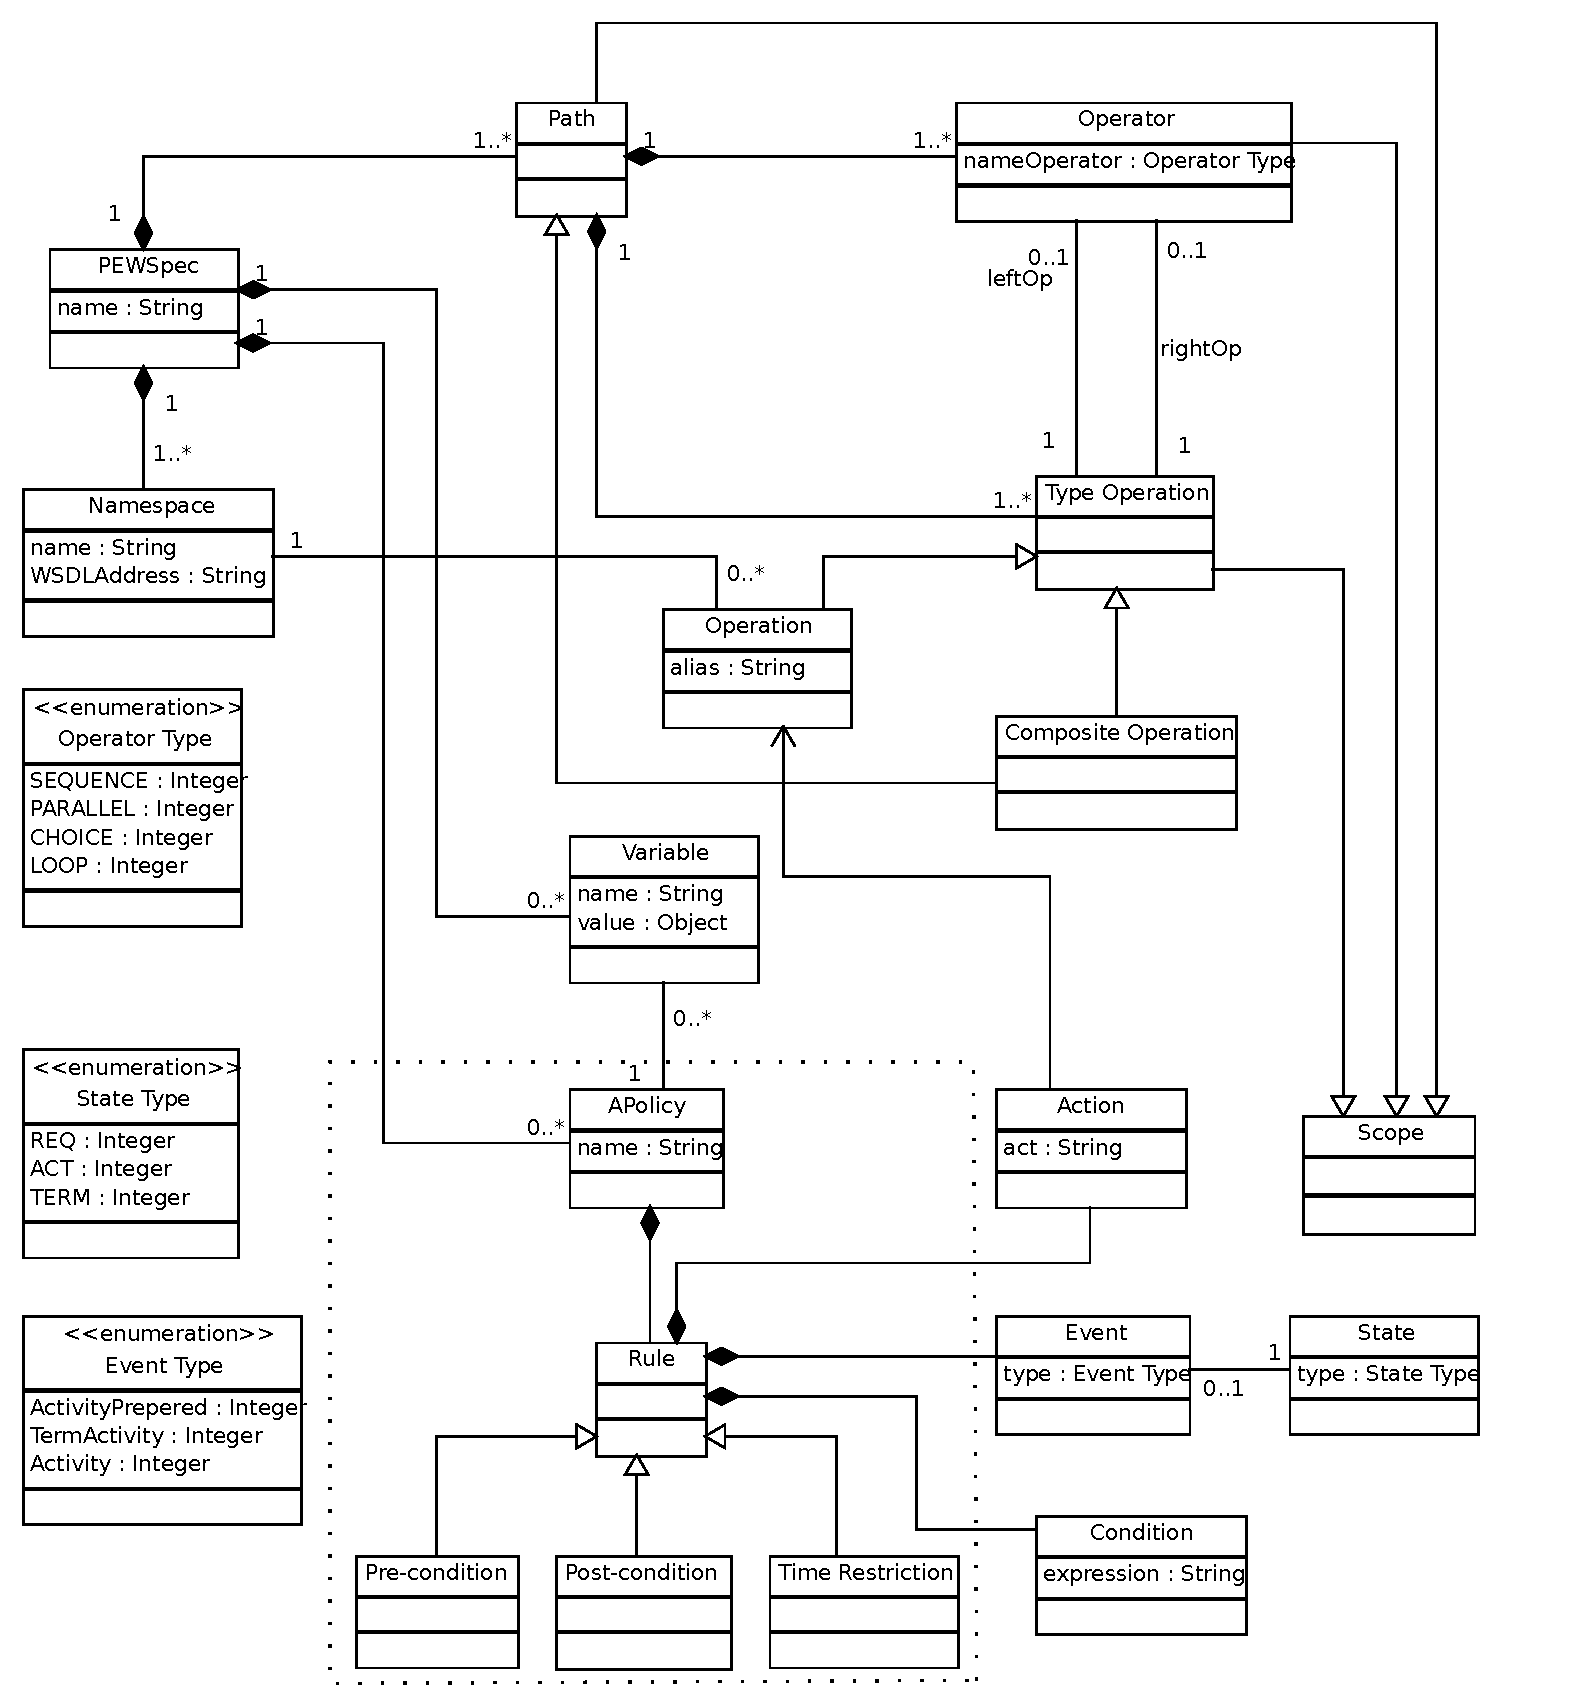
\includegraphics[width=1.0\textwidth]{figs/PEWSMetamodel}
%\caption{$\pi$-{\sc Pews} Metamodel}
%\label{fig:metamodel}
%\end{figure}
%%


The following example presents the \textit{$\pi$-PEWS} model for the ``To Publish Music'' application.

\begin{example}[To Publish Music (end)]\label{Colocar-o-label-correto-aqui}
The next code presents the \textit{$\pi$-PEWS}  model for our running example.\footnote{\color{red} Placido: Please change the pdf file as needed!}

\begin{center}
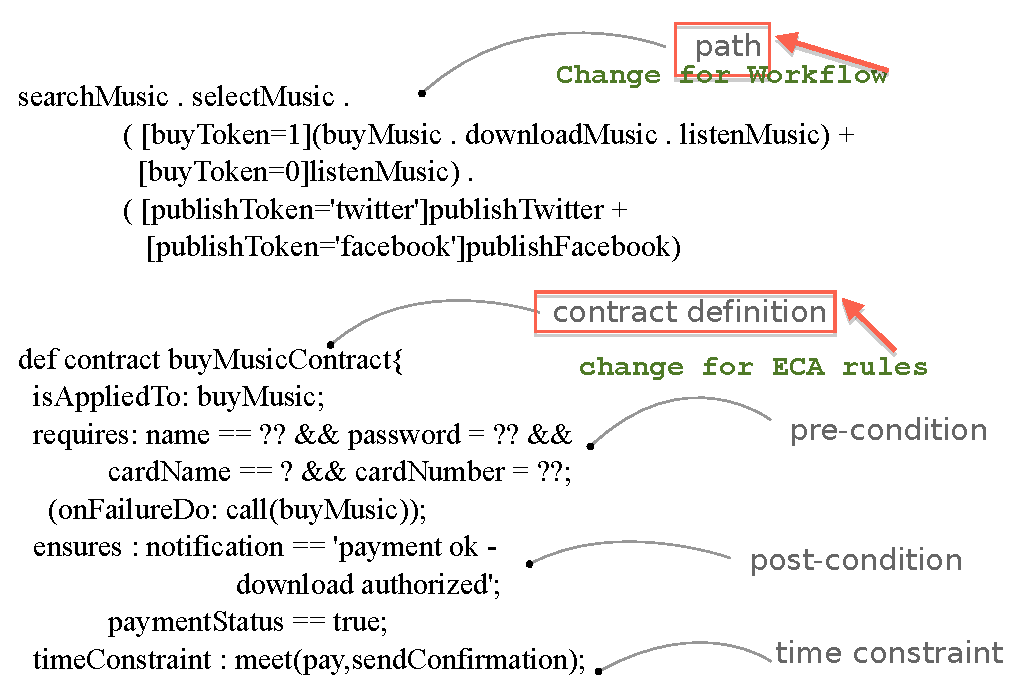
\includegraphics[scale=0.7]{figs/pewsEspecificationContract.pdf}
\end{center}

The upper part of the model consists of a workflow expression.
After the execution of searchSong, followed by selectSong,
the user may either buy, download and listen a song or just listen to a song (conditional workflow).
The last part of the wokflow publish the title of the song either on tweeter or facebook.

ECA rules are specified as ``contracts''.
In our case, the \texttt{buySongContract} specifies conditions to be verified when the \texttt{buySong} service is executed.
The contract specifies pre and post-conditions, as well as time constraints.\footnote{\color{red} Placido: Please verify the pre-condition assertions!}
The precondition\dots

In case of failure in verifying the precondition, the service \texttt{buySong} is retried.

The postcondition ensures that if the service completes, the payment is processed.

The time constraint indicates that the \texttt{sendConfirmation} service is invoked immediately after \texttt{buySong}.
\end{example}



===================================



Given a $\pi$-SCM model of a specific service based application (expressed according to the $\pi$-SCM meta-model), it is possible to generate its corresponding $\pi$-{\sc Pews} model. 
The following section describes the transformation rules between the $\pi$-SCM and $\pi$-{\sc Pews} meta-models.







The {\em A-policy} based service composition ($\pi$-SCM) meta-model, shown in Figure \ref{fig:e-scomposition-metamodel},
provides meta-classes to represent workflows\footnote{Workflows will be transformed into implemented service compositions.} that model  business processes.
The meta-model identifies {\sc Business Collaborators}\footnote{We use {\sc capitals} for referring to meta-model meta-classes.} and the {\sc Actions} they perform. 
Instances of this meta-model are represented as UML activity diagrams. 
In Figure~\ref{fig:e-scomposition-metamodel}  coloured boxes illustrate classes  modelling  non-functional properties and 
 white boxes represent classes modelling functional ones. 

%In the meta-model of Figure~\ref{fig:e-scomposition-metamodel}:
\begin{itemizedTrivlist}
\item A {\sc Business Collaborator} meta-class represents the classes of entities that collaborate in  business processes by performing some  required action. 
An instance of this meta-class is graphically represented as a partition in the activity diagram. 
A collaborator can be either internal or external to the system. 
When the collaborator of the business is external to the system, the attribute {\sf IsExternal}\footnote{We use the {\sf sans serif} font for referring to classes defined using a meta-model.} of the collaborator is set to \textbf{true}.

\item {\sc Action}s, a kind of {\sc ExecutableNode}, are represented in the model as a class activity instance of the meta-class Action. 
A class action represents some type of transformation or processing. 
There are two types of actions: i) a WebService (attribute Type is {\sf WS}); and ii) a simple operation called an {\sc ActivityOperation} (attribute Type is {\sc AOP}).
\begin{figure}[t]
\centering
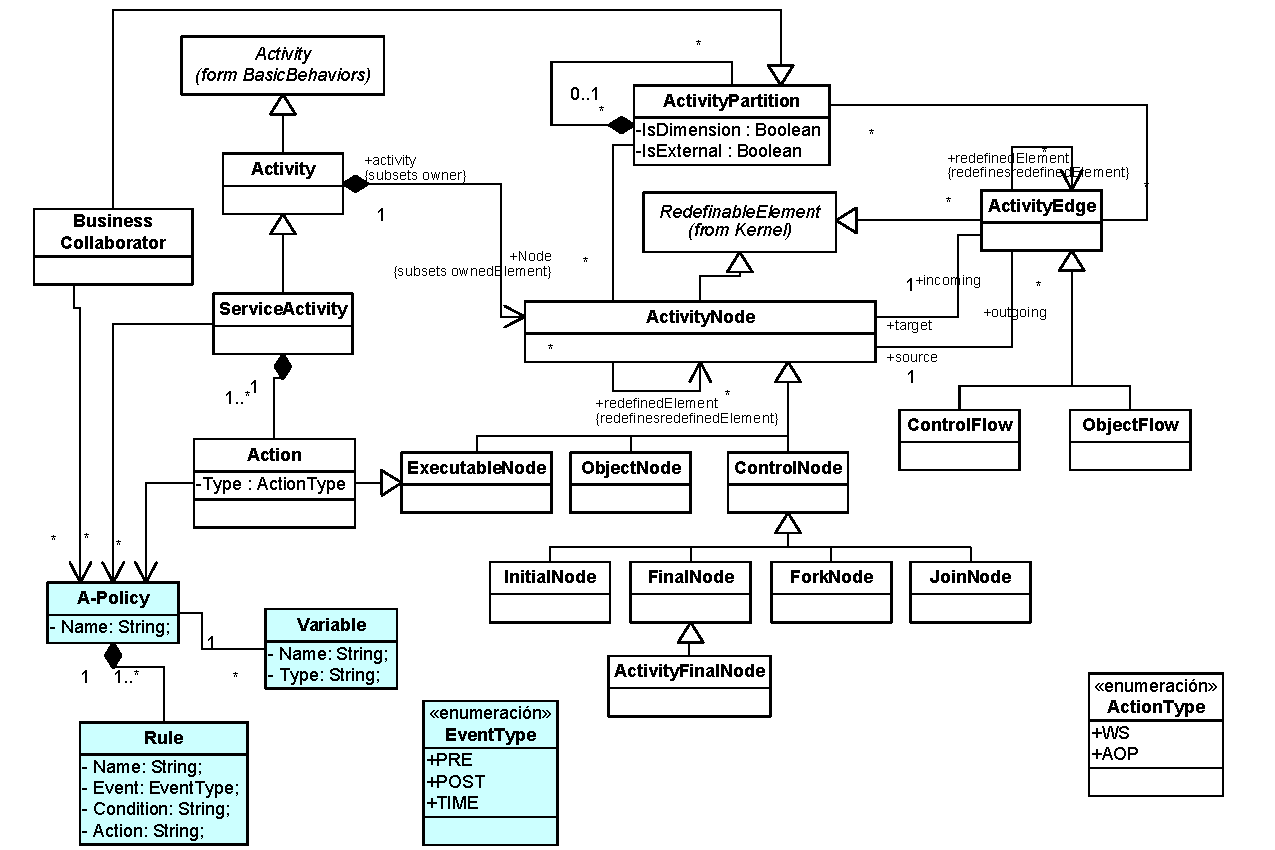
\includegraphics[width=1.0\textwidth]{figs/E-service-composition-metamodel}
\caption{$\pi$-Service Composition ($\pi$-SCM) Metamodel.}
\label{fig:e-scomposition-metamodel}
\end{figure}

\item The {\sc ServiceActivity} meta-class represents classes of composite activity types that must be carried out as part of a business service and is composed by one or more executable nodes.

\item In order to represent constraints types associated to services compositions, we extended introduced the meta-classes {\sc Rule} and {\sc A-policy} (see blue meta-classes in the $\pi$-SCM meta-model in Figure \ref{fig:e-scomposition-metamodel}).
We model non-functional constraints by using the notion of {\em A-policy}~\cite{Espinosa-Oviedo2011a,CIC:eovszmc09c}.
An {\em A-policy} is defined by attributes and rules. 
Intuitively, the conditions of each rule will be checked.
In case of no compliance, the actions defined by the rule will be performed.
The {\sc Rule} meta-class represents the types of event - condition - action rules where the {\sc Event} part represents the moment in which a constraint  will be evaluated.
An {\em A-policy} defines variables and operations that can be shared by the rules and that can be used for expressing their Event and Condition parts. 
\end{itemizedTrivlist}

\begin{figure}[t]%[htpb]
\centering
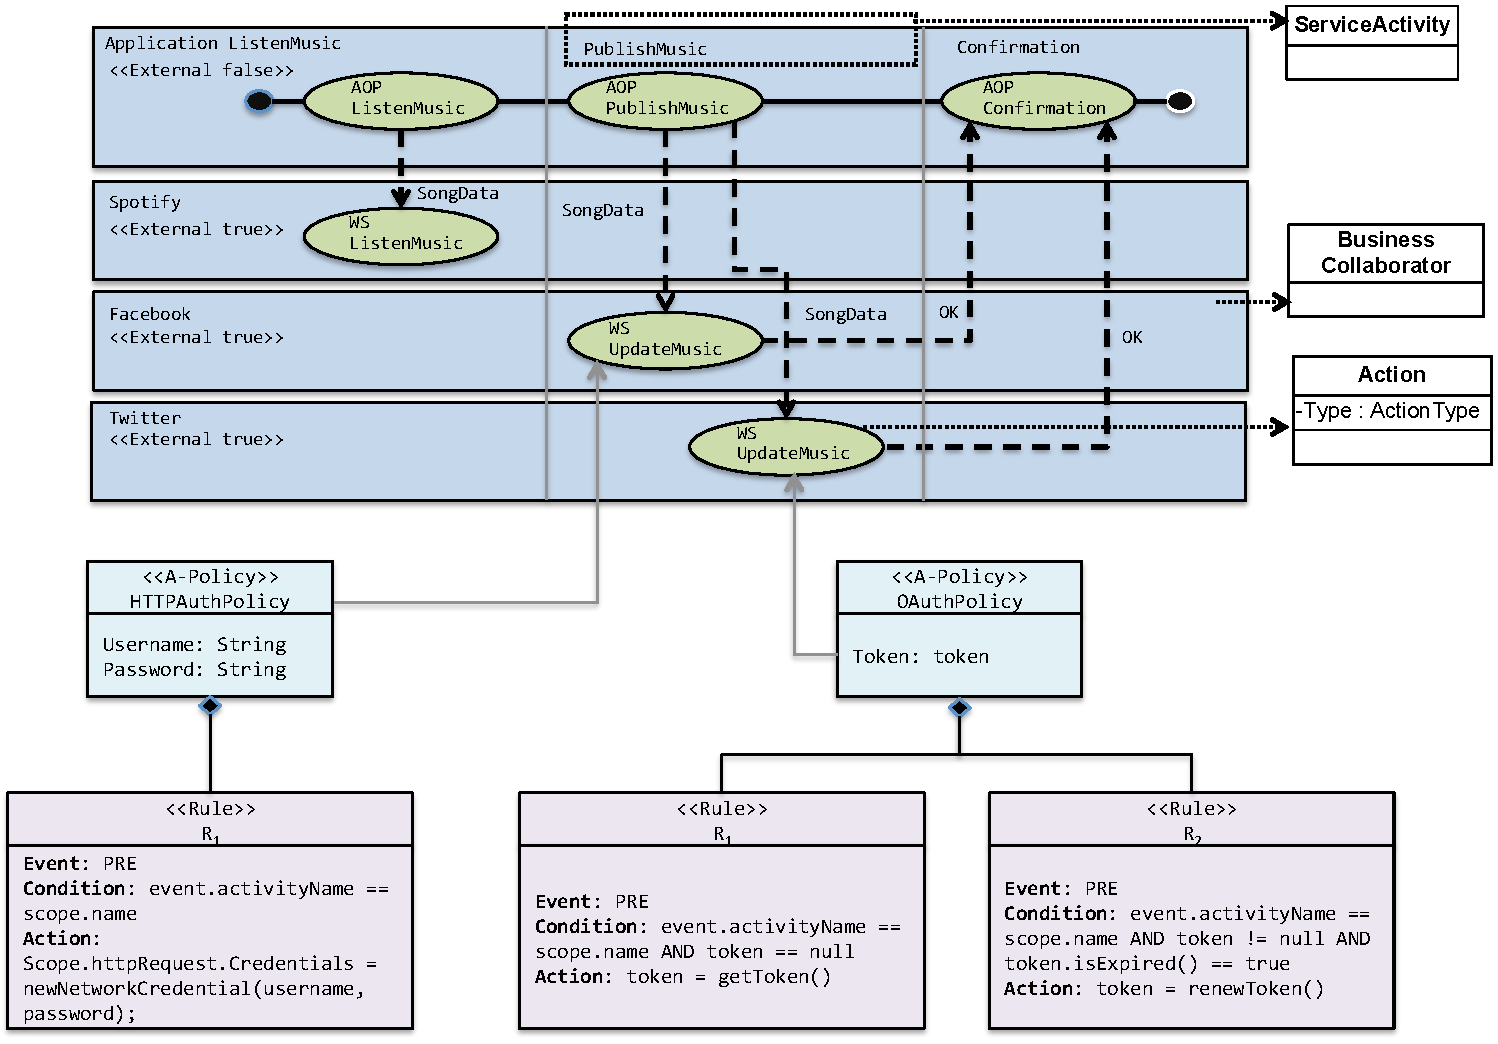
\includegraphics[width=0.95\textwidth]{figs/e-composition-model}

{\color{red}\LARGE PLACIDO: Please change the names of the boxes in accordance to the explanation --Martin}

\caption{$\pi$-SCM for the ``To publish music'' business service.}
\label{fig:servicecompositionmodel}
\end{figure}

\begin{example}[To Publish Music]\label{ex:toPublicMusic}
To illustrate the use of the $\pi$-Service Composition Meta-model, we define a model for the ``To Publish Music'' scenario (Figure \ref{fig:servicecompositionmodel}). 
In this model, there are three external business collaborators ({\em Spotify, Twitter} and {\em Facebook}).
% \footnote{We use {\em italics} to refer to concrete values of the classes of a model that are derived from the classes of a meta-model.}). 
The model also shows the business process of the application that consists of three service activities: {\em Listen Music}, {\em Publish Music} and {\em Confirmation}. 
Note that  the activity {\em Publish Music} calls the actions of two service collaborators namely {\em Facebook} and {\em Twitter}.
Both {\em Facebook} and {\em Twitter} services require authentication protocols in order to execute methods that will read and update the user space. 
%A call to such services must be part of the authentication protocol required by these services.
In the example we  associate two authentication policies, one for the open authentication protocol, represented by the class {\sf\small OAuthPolicy} at {\em Twitter}, that will be associated to the activity  {\sf\small UpdateTwitter} (see Figure \ref{fig:servicecompositionmodel}). 
In the same way, the {\em Facebook} class {\sf\small HTTPAuthPolicy}, for the http authentication protocol will be associated to the activity {\sf\small UpdateFacebook}.

{\sf\small OAuthPolicy} will implement the open authentication protocol.
The {\em A-policy} {\sf\small OAuthPolicy} has a variable {\sf\small Token} that will be used to store the authentication token provided by the service.
This variable is imported through the library {\sf\small OAuthPolicy.Token}. 
The A-policy {\sf\small OAuthPolicy} defines two rules, both can be triggered by events of type {\sf\small ActivityPrepared}: (R$_1$): If no token has been associated to the variable {\sf\small token}, then a token is obtained ; and (R$_2$): if the token has expired, then it is renewed. 
Notice that the code in the actions profits from the imported {\sf\small OAuthPolicy.Token} for transparently obtaining or renewing a token from a third party.

{\sf\small HTTPAuthPolicy} implements the HTTP-Auth protocol. 
The A-policy imports an http protocol library and it has two variables {\sf\small username} and {\sf\small password}.  
The event of type {\sf\small ActivityPrepared} is the triggering event of the rule {\sf\small R$_1$}. 
On the notification of an event of that type, a credential is obtained using the username and password. 
\hfill\openbox
\end{example}

We propose the use of rules and policies to model and associate non-functional properties to service compositions.
These artifacts will be used to generate the actual programs that will implement the application:
Once the $\pi$-Service Composition Model has been defined, then it can be transformed into a lower level model (in our case, $\pi$-PEWS) that gives support to code generation. 
The $\pi$-PEWS  meta-model is described in the next section. 


%..--..--..--..--..--..--..--..--..--..--..--..--..--..--..--..--..--..--..--..--..--..--..--..--..--..--..--..--..--..--..--..
\subsubsection{$\pi$-{\sc Pews}  meta-model}\label{sec:pewsmetamodel}
%..--..--..--..--..--..--..--..--..--..--..--..--..--..--..--..--..--..--..--..--..--..--..--..--..--..--..--..--..--..--..--..


This section  describes the $\pi$-SOD-M development environment that implements the generation of {\em A-policies}' based services' compositions. For a given services' based application, the process  consists in generating the  code starting from a $\pi$-SCM modeling an application. Note that the services' composition model is not modeled from scratch, but it is the result of a general process defined by the $\pi$-SOD-M method in which a set of models are built following a service oriented approach \cite{decastro1}.

%We used the Eclipse Modeling Framework (EMF) to implement the whole model transformation process \footnote {The EMF project is a modeling framework and code generation facility for building tools and other applications based on a structured data model.}. From a model specification described in XMI, EMF provides tools and runtime support to produce a set of Java classes for the model, along with a set of adapter classes that enable viewing and command-based editing of the model, and a basic editor.
%In order to automate the transformation we specified  transformation rules using the ATL model transformation language Finally, in order to generate code we  used Acceleo \footnote{http://www.acceleo.org/pages/home/en}.

%%..--..--..--..--..--..--..--..--..--..--..--..--..--..--..--..--..--..--..--..--..--..--..--..--..--..--..--..--..--..--..--..--..--..--..--..--..--..--
%\subsection{$\pi$-SOD-M Development Environment}
%%..--..--..--..--..--..--..--..--..--..--..--..--..--..--..--..--..--..--..--..--..--..--..--..--..--..--..--..--..--..--..--..--..--..--..--..--..--..--

Figure \ref{fig:policymanager} depicts a general architecture of the $\pi$-SOD-M Development Environment showing the set of plug-ins  developed in order to implement it. The environment implements the abstract architecture. Thus, it consists of plug-ins implementing the $\pi$-SCM and $\pi$-{\sc Pews} meta-models used for defining models specifying services' compositions and their associated policies; and ATL rules for transforming  PSM models (model to model transformation) and finally generating code (model to text transformation).
\begin{figure}[htpb]
	\begin{center}
		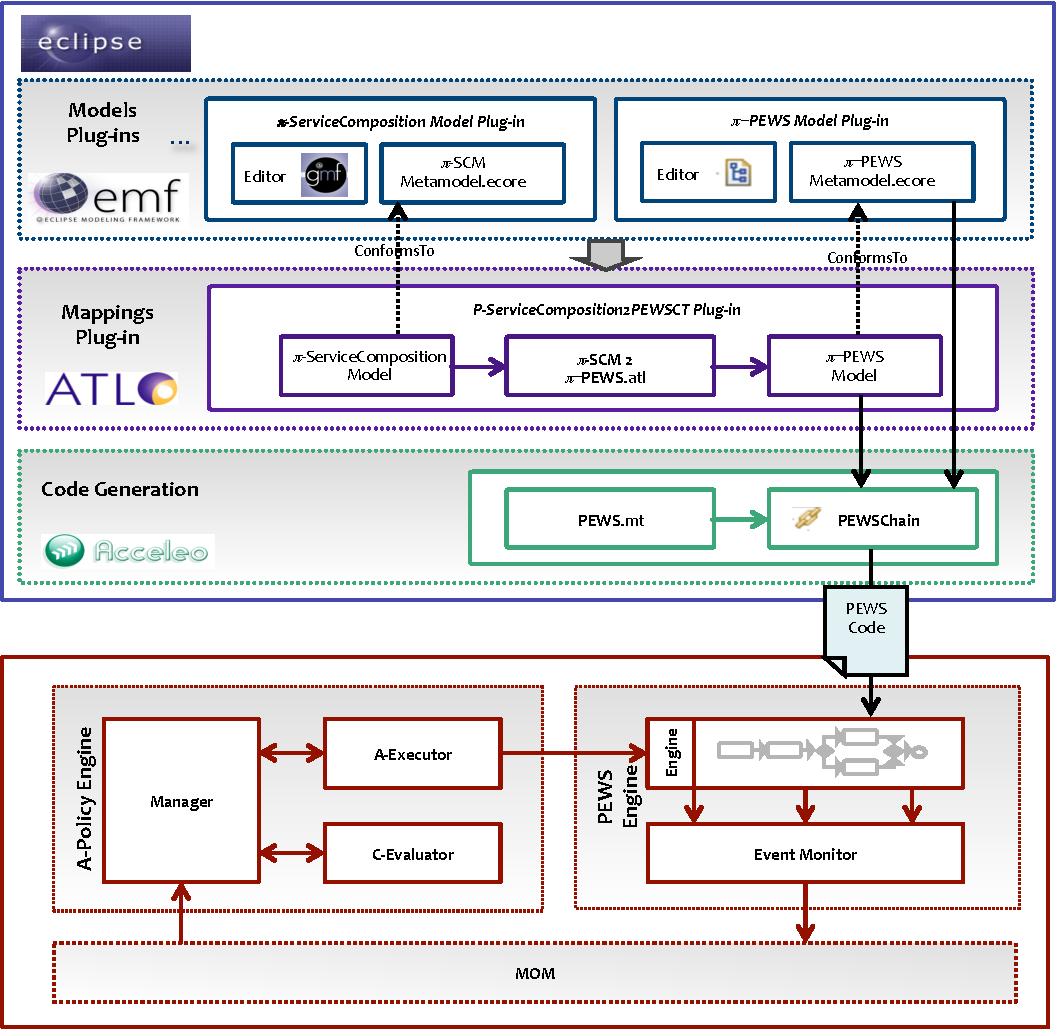
\includegraphics[width=0.60\textwidth]{figs/architecture}
	\end{center}
		\caption{$\pi$-SOD-M Development Environment}
   \label{fig:policymanager}
\end{figure}
\begin{itemize}
\item 	We  used the Eclipse Modeling Framework (EMF) \footnote {The EMF project is a modeling framework and code generation facility for building tools and other applications based on a structured data model.}   for implementing the meta-models  $\pi$- SCM and $\pi$-{\sc Pews}. Then, starting form these meta-models, we  developed the models' plug-ins needed to support the graphical representation of the $\pi$- SCM and $\pi$-{\sc Pews} models ($\pi$-ServiceCompostion Model and $\pi$-PEWS Model plug-ins).

\item	 We used  ATL \footnote{http://eclipse.org/atl/. An ATL program is basically a set of rules that define how source model elements are matched and navigated to create and initialize the elements of the target models.}
for  developing the mapping plug-in implementing the  mappings between models ($\pi$-ServiceComposition2$\pi$-PEWS Plug-in).

\item 	We  used Acceleo \footnote{http://www.acceleo.org/pages/home/en} for implementing  the code generation plug-in. We coded the pews.mt program  that implements the model to text transformation for generating executable code. It takes as input a $\pi$-PEWS model implementing a specific services' composition and it generates the code to be executed by the 
{\em A-policy} based services' composition execution environment. 

%\item Finally, we created a chain execution  to execute the model to text transformation.
\end{itemize}

%
As  shown in Figure \ref{fig:policymanager}, once an instance of a PEWS code is obtained starting form a particular $\pi$-services' composition model it can be executed over {\em A-policy} based services' composition execution environment  consisting of a composition engine and a {\em A-policy} manager.  The  {\em A-policy} manager  consists of three main components Manager, for scheduling the execution of rules, C-Evaluator and A-Executor respectively for evaluating rules' conditions and executing their actions. The {\em A-policy} Manager interacts with a composition engine thanks to a  message communication layer (MOM).


The composition engine manages the life cycle of the composition. Once a composition instance is activated, the engine schedules the composition activities according to the composition control flow.
Each activity is seen as the process where the service method call is executed.
The execution of an activity has four states: prepared, started, terminated, and failure.
The execution of the control flow (sequence, and/or split and join) can also be prepared, started, terminated and raise a failure.

At execution time, the evaluation of policies done by the {\em A-policy} manager must be synchronized with the execution of the services' composition (i.e., the execution of an activity or a control flow).  Policies associated to a scope are activated when the execution of its scope starts. A {\em A-policy} will have to be executed only if one or several of its rules is triggered. If several rules are triggered the {\em A-policy} manager first builds an execution plan that specifies the order in which such rules will be executed according to the strategies defined in the following section. 
%Once rules have been executed, the {\em A-policy} finishes its execution and returns to a sleeping state.
If rules belonging to several policies are triggered then policies are also ordered according to an execution plan. The execution of policies is out of the scope of this paper, the interested reader can refer to \cite{Espinosa-Oviedo2011a} for further details.
%The order of policies has implications on the global order of the rules to be executed.
















=============================================================================

We validated our methodology by developing a use-case concerning risk assessment for financial companies.
Our application is inspired on the ORCA System\footnote{The ORCA System is a trademark of GCP Global (www.gcpglobal.com).}.
Risk assessment is implemented by an interactive business process based on the exchange of a series of questionnaires intended to evaluate the risks implied the client's business practice.
For instance, the conditions and protocols used to perform confidential transactions, the physical security for accessing reserved areas such as computing server installations.
The information gathered by the questionnaires is used to determine whether there are risky practices within the business processes of the company, as well as to propose amends to these practices.
The ultimate goal of the risk assessment is to determine a degree of compliance to existing standards.
By analysing the questionnaires, ORCA detects risky practices, proposes solutions and triggers further assessment processes to ensure that the solutions have been implemented.

Our goal is to model a service based application (called \FlyingPig), for providing risk assessment as a service.
In order to provide this functionality, \FlyingPig\ would benefit from ORCA's legacy services: storage, assessment and data visualization functions.

In the following, we describe the results of applying $\Pi$-SODM to develop the \FlyingPig\ risk assessment system.
The models presented next were generated as a result of interacting with software developers at GCP Global.

\begin{figure}
\centering
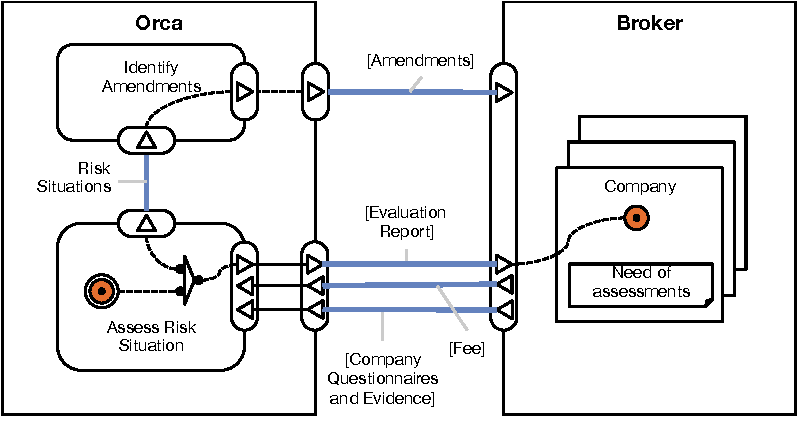
\includegraphics[width=0.7\textwidth]{figs/3ValueModel.pdf}
\hspace*{5cm}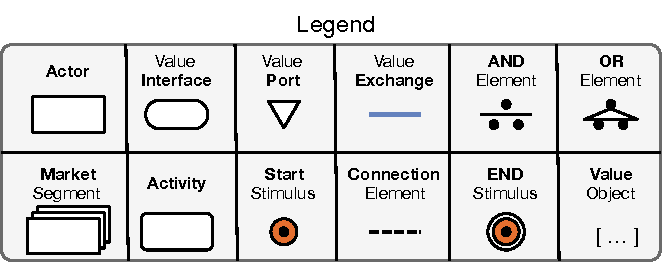
\includegraphics[width=0.4\textwidth]{figs/3ValueKey.pdf}
\caption{E3value model for \FlyingPig.\label{fig:E3valuemodel}}
\end{figure}


\subsection{Computation-Independent Models (CIM)}

Figure~\ref{fig:E3valuemodel} shows the value model for the \FlyingPig\ application.
It is a business model that graphically represents a business case as a set of value exchanges ($\triangleright$ and $\triangleleft$) and value activities (rounded boxes) performed by business actors (squared boxes).

In our use-case, we identify two business actors: \textsl{ORCA} and \textsl{Broker}. 
Brokers are responsible for channelling requests for risk assessment of one or several companies. 
ORCA have two value activities which are services that provide an economical benefit: to \textsl{Identify Amendments} and the possibility to \textsl{Assess Risk Situation}. 
The values exchanged between ORCA and the brokers are: \textsl{Amendments} and \textsl{Evaluation Reports} which are value objects ([ \!\dots]) for the companies that need to have a risk assessment, as well as  \textsl{Questionnaire and Evidences} and the risk assessment \textsl{Fee} which are value objects for ORCA System.



The dependency path in Figure~\ref{fig:E3valuemodel} initiates with the need of assessment by a particular company. 
Once this need occurs, the value exchanges between ORCA and Broker are triggered. 
The client company will provide orca wit information (answers to a questionary), evidence (to support the information) and a fee (monetary value).
ORCA will provide amendments (recommendations to change practices) and an evaluation report. 

\begin{figure}[t]
\centering
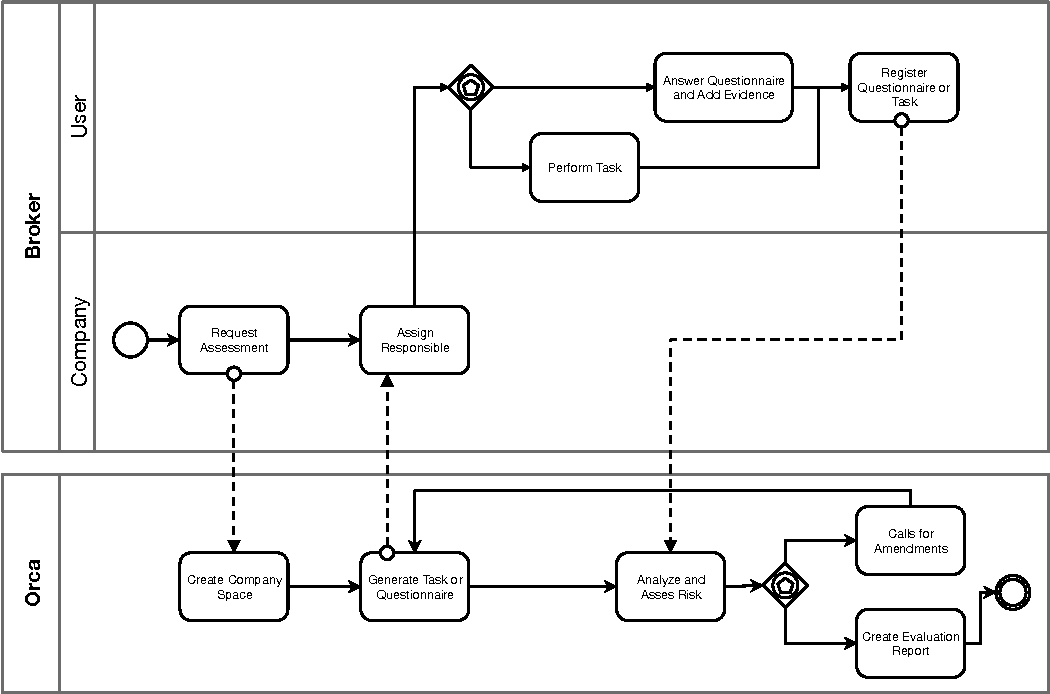
\includegraphics[width=1.0\textwidth]{figs/BPMN_GCP.pdf}

{\color{red} Javier: Please change \underline{Asses} by \underline{Assess}. --M}
\caption{BPMN model for \FlyingPig.\label{fig:BPMNmodel}}
\end{figure}

The BPMN model is devised to better understand the process in which the value exchanges occur.
Figure~\ref{fig:BPMNmodel} shows the BPMN model\footnote{Details on BPMN (Business Process Management Notation) can be found in http://www.bpmn.org/.} for the \FlyingPig\ scenario. 
The model includes two pools representing the \textsl{ORCA} system and the \textsl{Brokers}. 
Brokers have two lanes, the client \textsl{Company} and a \textsl{User}. 
The user is a contact member of the company, who will coordinate the assessment process. 
This process will involve other members of the company as well.

The risk assessment process starts after a request from a company.
(This agrees with the value model, in which the start stimulus triggers the whole process.)
The request leads to the definition of a group of users that will answer questionnaires for evaluating risk.
Questionnaires are considered tasks that users will have to perform. 
Other tasks include amending a ``risky situation'' as well as producing evidence to show that a specific risk has been eliminated\footnote{Risky situations include from physical facts such as not having easy access to handicapped persons or having an unsecured access to the premises of the company, to more intangible ones, such as the use of an less-than-optimal protocol to access data on the company's computer server.}.

Once tasks are completed, they are stored and analysed to generate a list of un-compliant situations, associated to their corresponding \textit{calls for amendment}, in case there are any, or a report specifying a compliance level, incidents and a risk map.
During the process of analysing a questionnaire, the answers of some questions can trigger the generation of other questionnaires or amendments, that will become new tasks.  

Business processes have also associated rules and constraints that define their non functional requirements.
NFR represents the ``semantics'' and the conditions in which the tasks must be done.
In our example we have some constraints.

{\color{red}
Placido, Valeria: What can we say about non-functional requirements at the CIM level?
}

\subsection{Platform-Independent Models (PIM)}

In Section~\ref{sec:modelingWithPISODM} we defined three models at the PIM level.
These models are built next, for the \FlyingPig\ scenario.

\begin{figure}[t]
\centering
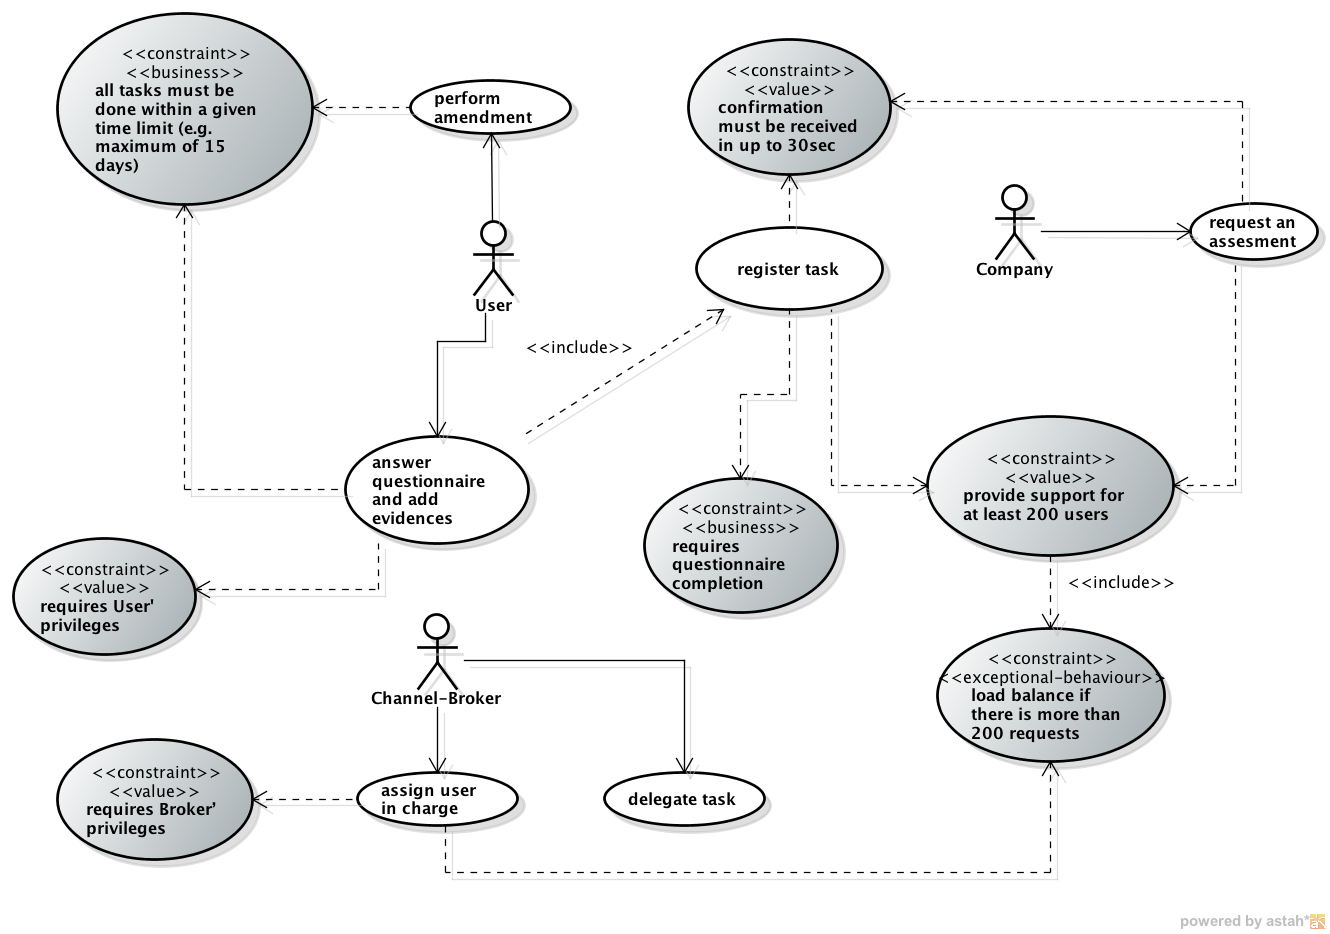
\includegraphics[width=0.9\textwidth]{figs/UseCaseGeneral.png}

{\color{red} \raggedright
$\star$ ``Create a responsible'' should be changed for ``Designate user in charge''.

$\star$ ``requires concurrency for more than 200 users'' should be changed by ``Maximum number of users should be greater than 200''.
}
\caption{$\pi$-UseCase model for \FlyingPig.\label{fig:piUseCaseModel}}
\end{figure}


\paragraph{\underline{$\pi$-UseCase Model for \FlyingPig}}~

The $\pi$-UseCase model shown in Figure~\ref{fig:piUseCaseModel} describes the features and constraints for the \FlyingPig\ application. 
In this model, three actors are identified: \textit{Company}, \textit{User} and \textit{Channel-Broker}\footnote{\color{red} Can we change this for Broker ? --M.}. 
They are represented as stick figures.
In the context of \FlyingPig, Company is the actor asking for risk evaluation.
A Channel-Broker is the responsible for channelling the the evaluation process, assigning users to be in charge of tasks as well as delegating tasks. 
A User, in this model is an actor who answers questionnaires (with base on the actual facts about the Company).
The User also produces evidence to support facts and performs the necessary amendments to improve the results of the risk assessment.

Each actor is associated to one or more use cases (depicted as white ovals in Figure~\ref{fig:piUseCaseModel}). 
Use cases describe the main functionalities of the system.
The $\pi$-UseCase model for \FlyingPig\ defines six use cases. 

In our model, each use case may be associated to one or more (non-functional) constraints (depicted as coloured ovals in Figure~\ref{fig:piUseCaseModel}). 
The model defines three types of constraints: \textit{value} , \textit{business} or \textit{exceptional behavior}. 
Each constraint is identified by the word $<<$\textsf{constraint}$>>$ followed by its type.

In the case of \FlyingPig, the model counts seven constraints:
\begin{numtrivlist}
\item An acknowledgement is due less than 30 seconds after registering a task or demand for assessment. 
\item The system's infrastructure should be prepared to deal with, at least, 200 users. 
\item If the number of requests exceeds 200, \FlyingPig\ should make a load balance of the requests. 
\item The Channel-Broker must have their privileges verified \textit{before} the execution of the actions associated to the \textsf{designate user in charge} use case.
\item Users must have their privileges verified \textit{before} the execution of the actions associated to the \textsf{answer questionnaire and add evidences} use case.
\item All questionnaires need to be fully answered, in order to consider that a task is completed.
\item There is a time limit (in days) for each amendment required by the system.
\end{numtrivlist}

{\color{red} Anything else here? --M}

\begin{figure}
\centering
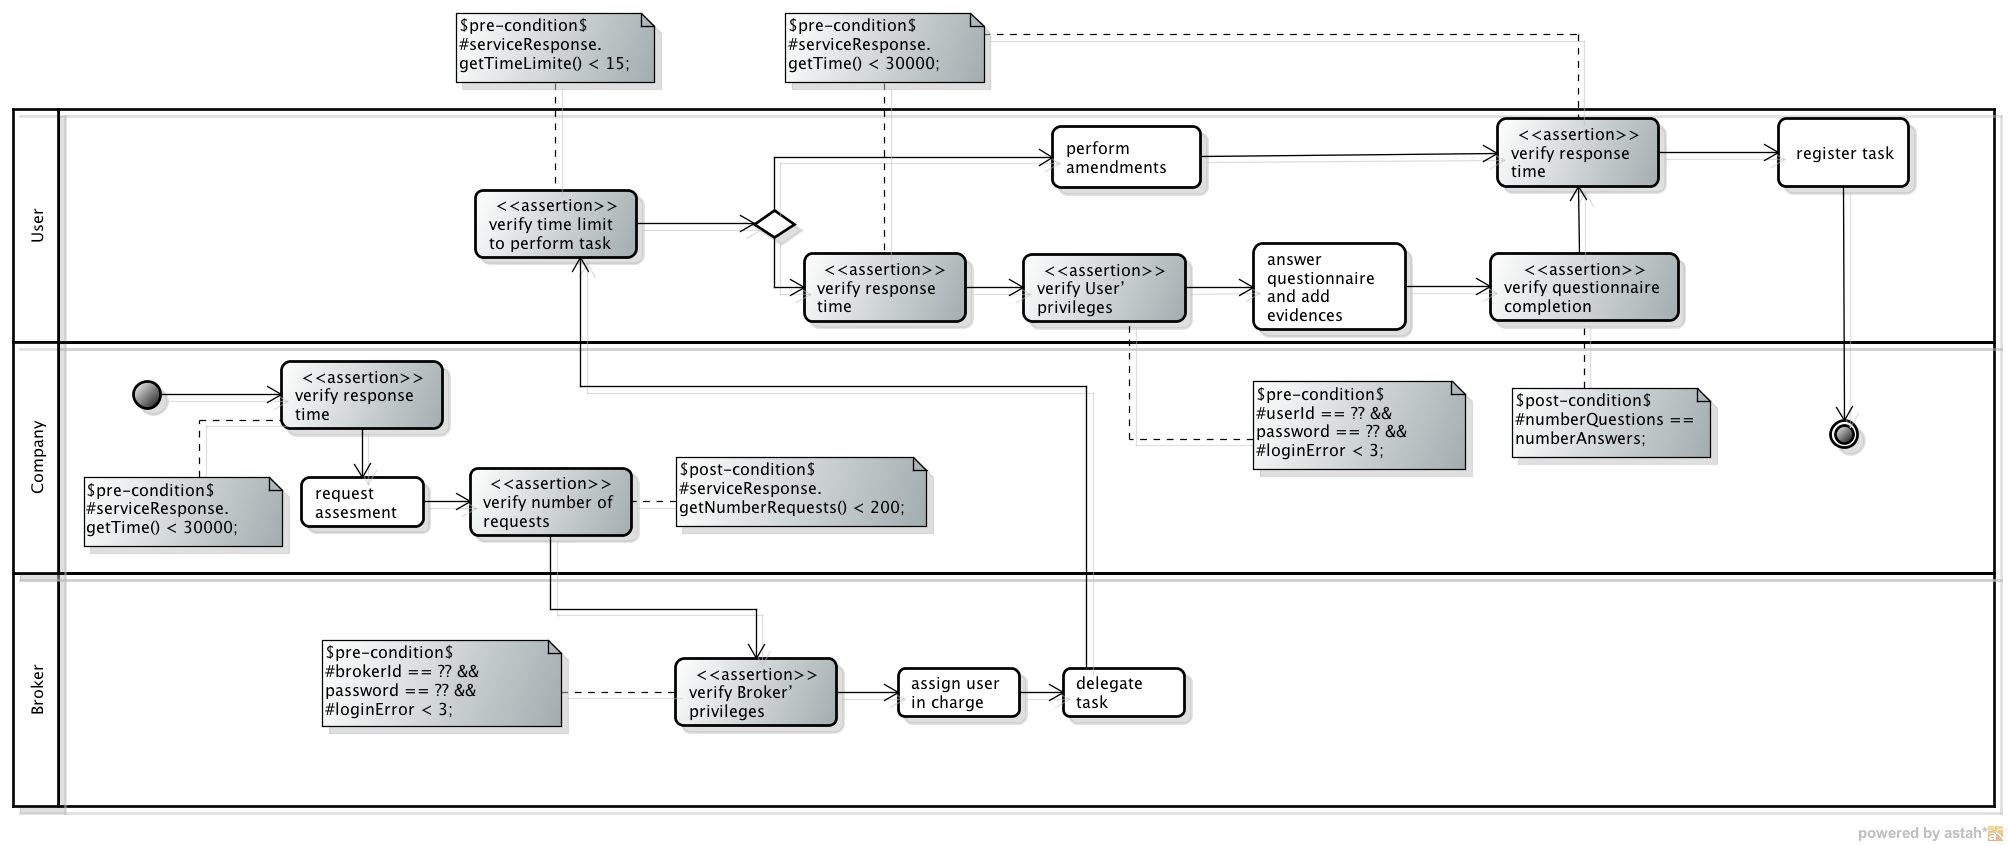
\includegraphics[width=1.0\textwidth]{figs/ServiceProcessGeneralCut.png}
\caption{$\pi$-ServiceProcess model for \FlyingPig.\label{fig:PiServiceProcessModel}}
\end{figure}

\paragraph{\underline{$\pi$-ServiceProcess Model for \FlyingPig}}~

The $\pi$-ServiceProcess model (Figure~\ref{fig:PiServiceProcessModel}) presents the workflow for \FlyingPig.
The actions in this model were obtained by applying the use case transformation rules described in Section~\ref{sec:pewsmetamodel}.

The \textsf{Company}, \textsf{Broker-Channel} and \textsf{User} actors are transformed into lanes that represent the business collaborators.
Use cases are transformed into \textit{actions} and are represented by white boxes.
The restrictions associated to each use case are transformed into \textit{assertions} (represented by coloured boxes) and may be decorated with pre- and post-conditions. 
We can see that this model refines the concepts defined in the $\pi$-UseCase model.
The assertions specify those non-functional requirements, as they are seen by the actors. 
The next step in the development is to add these assertions to the models that specify the \FlyingPig\ system.

\begin{figure}[t]
\centering
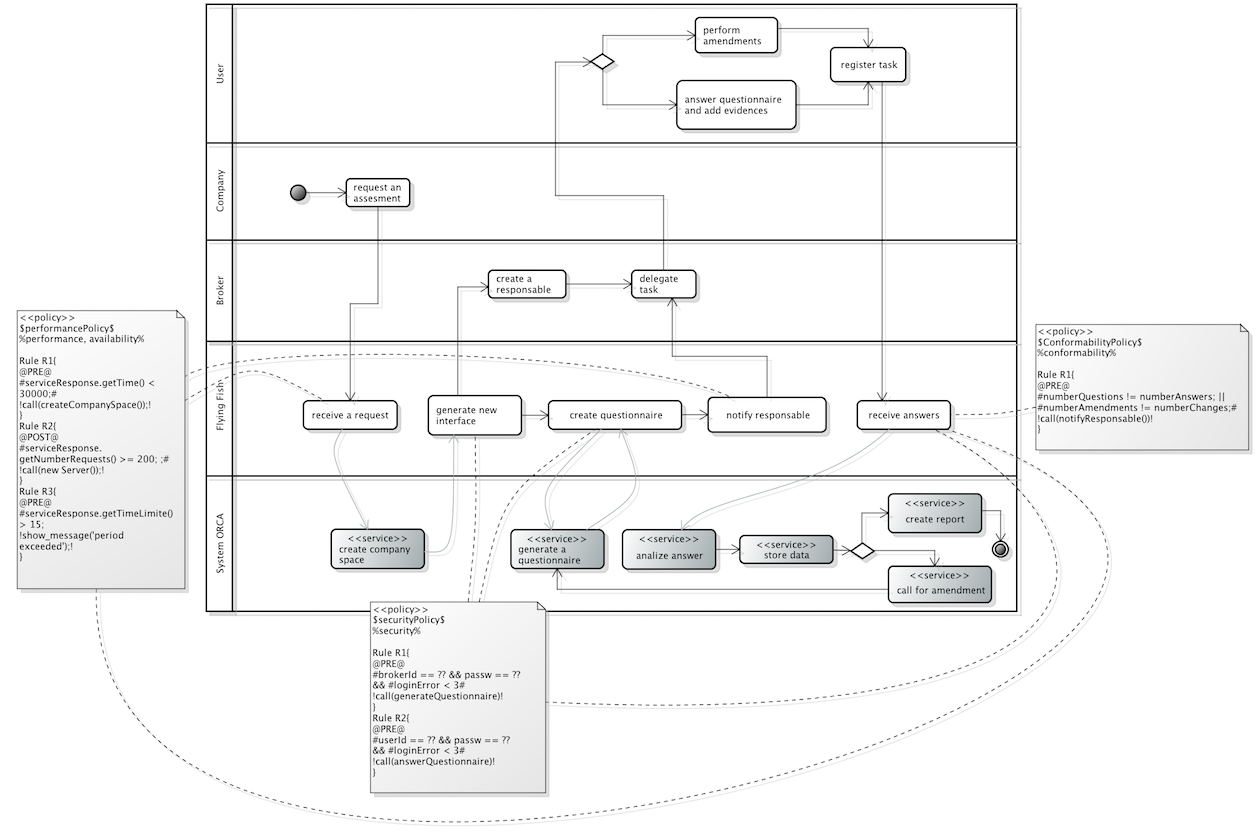
\includegraphics[width=1.0\textwidth]{figs/ServiceCompositionGeneralCut.png}
{\color{red} \raggedright
$\star$ Change FlyingFish by \FlyingPig.
}
\caption{$\pi$-ServiceComposition model for \FlyingPig.\label{fig:PiServiceCompositionModel}}
\end{figure}

\paragraph{\underline{$\pi$-ServiceProcess Model for \FlyingPig}}~

The model presented in Figure~\ref{fig:PiServiceCompositionModel} offers a system-centric view of the application.
The previous model is now enhanced with a view of the \FlyingPig\ application, including those services upon  it is build.
The assertions in Figure~\ref{fig:PiServiceProcessModel} are implemented as \textit{policies}.
These policies contain the pre- and post-conditions of the previous model.
They are associated to actions of the system.


%\begin{figure}[t]
%\centering
\begin{lstlisting}[label=list:flyingPigPiPEWS,caption=pi-PEWS
Specification: FlyingPig. ]!\label{fig:PiPEWSModel}!

//Namespaces specify service URI
namespace orca = www.orca.mx/service.wsdl

//Operations
alias createCompanySpace = portType/createCompanySpace in orca
alias generateQuestionnaire = portType/generateQuestionnaire in orca
alias analizeAnswer = portType/analizeAnswer in orca
alias storeData = portType/storeData in orca
alias createReport = portType/createReport in orca
alias callForAmendments = portType/callForAmendments in orca

//Services
service receiveRequest(R, Id) = createCompanySpace(R, Id)

service generateNewInterface(Id, NULL) = ...

service createQuestionnaire(Id, Q) = generateQuestionnaire(Id, Q)

service notifyResponsable((Id, Q); NULL) = ...

service receiveAnswers((Id, T); P) =
			analizeAnswer((Id, T), NULL) 
			. storeData((Id, T), NULL)
			. (
			  (createReport(Id, P) . return(P))
			  + (callForAmendments(Id,T) . return(NULL))
			  )
  
//Path

receiveRequest(R, Id)
||
( generateNewInterface(Id, NULL)
  . createQuestionnaire(Id, Q)
  .  notifyResponsable((Id, Q); NULL
 )
||
 ( receiveAnswers((Id, T); P)
 . [P != NULL] STOP
 )*	
 
//Policies 					  


\end{lstlisting}
%\fbox{\LARGE $\pi$-PEWS Model.}
%
%{\color{red} \raggedright
%$\star$ Placido: Please, place the model here.
%}
%\caption{$\pi$-PEWS model for \FlyingPig.\label{fig:PiPEWSModel}}
%\end{figure}

\subsection{Platform-Specific Model (PSM)}

The model presented in Figure~\ref{fig:PiPEWSModel} is the result of translating the previous model into service composition code.
Notice that the workflow for \FlyingPig\ is implemented by using the constructors present in BPEL~\cite{BPEL}, with the addition of the notion of \textit{contract}.

Contracts may be implemented as transversal concerns~\cite{aspects}.
Their conditions may be verified at specific point of the composition and their actions are executed if needed.

%%%%%%%%%%%%%%%%%%%%%%%%%%%%%%%%%%%%%%%%%%%%%%%%%%%%%
\subsection{Lessons Learned}

Through the example we underlined that every application implements functional aspects that describe its application logic.
Recall that an application logic refers to routines that perform the activities to reach the application objective.
Also there are non functional properties derived from NFR. They refer to strategies to be considered for the application execution like: security, isolation, adaptability, atomicity, and more.
These non functional properties must be ensured at execution time, and they are not completely defined within the application logic.

The challenge is to define them and to associate them with the application logic considering that different to existing solutions that suppose that it is possible to access the execution stat of all the components  of an application and that the application has complete control on them, in the case for service oriented applications  the components are autonomous services
API does not necessarily export information about methods dependency (e.g., in the REST protocol);
they do not share their state (stateless).

Given a set of services with their exported methods known in advance or provided by a  service directory, building services' based applications can be  a simple task that implies expressing an application logic as a services' composition. The challenge being  ensuring the compliance between the specification and the resulting application. Software engineering methods (e.g., \cite{1,2,decastro1,PapazoglouH06}) today can help to ensure this compliance, particularly when information systems include several sometimes complex business processes calling Web services or legacy applications exported as services.

As WS-* and similar approaches, our work enables the specification and programming of crosscutting aspects (i.e., atomicity, security, exception handling, persistence).
In contrast to these approaches, our work specifies policies for a services composition in an orthogonal way. Besides, these approaches suppose that non-functional properties are implemented according a the knowledge that a programmer has of a specific application requirements but they are not derived in a methodological way, leading to ad-hoc solutions that can be difficult to reuse. In our approach, once defined the policies for a given application they can be reused and/or specialized for another one with the same requirements or that uses services that impose the same constraints.